\documentclass{beamer}
\usetheme{Szeged}
\definecolor{beamer@andja}{rgb}{0.5, 0.7, 0.4}
\setbeamercolor{structure}{fg=beamer@andja}	
\usepackage{beamerthemeshadow}
\usepackage{url}
\usepackage[utf8]{inputenc}
\usepackage{graphicx}
\usepackage{color}

\setbeamertemplate{footline}{\hspace*{.5cm}\scriptsize{\hspace*{50pt} \hfill\hspace*{.5cm}}\\
\vspace{9pt}}

\usepackage[english,serbian]{babel}

\begin{document}
\title{\Large Detekcija zajednica u socijalnim mrežama\\ \scriptsize {Seminarski rad u okviru kursa\\Računarska inteligencija}\\ \vspace{5pt}\tiny{profesor: Aleksandar Kartelj \\asistenti: Stefan Mišković, Denis Aličić}}
\institute {Matematički fakultet\\}
\author{Aleksandra Nikšić \hspace{5ex} Anđelka Milovanović\\ \tiny mi16072 \hspace{35ex} mi15145}
\date{\scriptsize 25. april 2020.}

\setbeamertemplate{footline}
{
  \leavevmode
  \hbox{
  \begin{beamercolorbox}[wd=.5\paperwidth,ht=2.25ex,dp=1ex,center]{author in head/foot}
    \usebeamerfont{author in head/foot}{Anđelka Milovanović, Aleksandra Nikšić}
  \end{beamercolorbox}
  \begin{beamercolorbox}[wd=.48\paperwidth,ht=2.25ex,dp=1ex,center]{title in head/foot}
    \usebeamerfont{title in head/foot}{Detekcija zajednica u socijalnim mrežama}
  \end{beamercolorbox}}
}

\begingroup
\setbeamertemplate{footline}{}
\begin{frame}
  \titlepage
\end{frame}
\endgroup

\setbeamertemplate{section in toc}[sections numbered]
\setbeamertemplate{subsection in toc}[subsections numbered]
\setbeamerfont{subsection in toc}{size=\footnotesize}

\begin{frame}\frametitle{Sadržaj}\tableofcontents
\end{frame} 


\section{Uvod} 
\subsection{Motivacija}
\begin{frame}\frametitle{Motivacija}
\begin{itemize}
    \item Zašto je detekcija zajednica važna?
        \begin{itemize}
            \item uočavanje strukture mreže
        \end{itemize}
    \item Koji problemi postoje?
        \begin{itemize}
            \item posmatramo samo eksplicitne veze između čvorova
            \item pronalazak jače i slabije povezanih delova mreže
        \end{itemize}
    \item Gde se može primeniti?
    U disciplinama u kojima su sistemi predstavljeni kao grafovi
        \begin{itemize}
            \item sociologija
            \item biologija
            \item računarstvo
        \end{itemize}
\end{itemize}
\end{frame}

\section{Algoritmi} 
\begin{frame}\frametitle{Različiti pristupi}
\begin{itemize}
    \item Pristupi
        \begin{itemize}
            \item detektovanje i uklanjanje grana sa ciljem razdvajanja klastera
            \item genetski algoritmi, gde su jedinke nizovi čvorova sa određenim pripadnostima
        \end{itemize}
    \item Naš pristup
    \begin{itemize}
            \item GN sa gustinskom modularnošću
            \item MemeNet sa heuristikom simuliranog kaljenja umesto lokalne pretrage
        \end{itemize}
\end{itemize}
\end{frame}

\subsection{Girvan-Newman}

\begin{frame}\frametitle{Girvan-Newman Q}
\begin{itemize}

\item klasična modularnost za GN: \begin{equation} Q = \frac{1}{2m} \sum_{ij}{}(A_{ij} - P_{ij}) \delta(C_{i}, C_{j})
\end{equation}
\item \textbf{naš pristup} za GN sa gustinskom modularnošću: \begin{equation} D = \sum_{i = 1}^{m} \frac{L(V_{i},  V_{i}) - L(V_{i}, \overline V_{i})}{|V_{i}|} 
\end{equation}
\end{itemize}
\end{frame}

\begin{frame}\frametitle{Girvan-Newman}

\begin{enumerate}
\item postavi se najbolja modularnost na BestQ=0
\item učita se graf i izračunaju se njegove komponente
\item izračuna se edge-betweenness za sve ivice i obrišu se sve one sa maksimalnom vrednošću (one su most između zajednica)
\item izračuna se novi broj komponenti grafa
\item ako je novi broj komponenti $\leq$ od početnog onda se ponavlja korak 3
\item izračuna se modularnost i sačuva se u Q
\item ako je Q$>$BestQ onda se ažurira najbolja modularnost i sačuva se ta podela grafa kao najbolja u BestComps 
\item ako nema više ivica u grafu vraća se BestComps, u suprotnom se ponavlja proces od koraka 3 na dalje
\end{enumerate}

\end{frame}

\subsection{Meme-Net}
\begin{frame}\frametitle{Meme-Net}
    \begin{itemize}
        \item rekombinacija gena + pojedinačne optimizacije
        \item optimizacija gustinske modularnosti
        \item podesivi parametar $\lambda$
        \item simbioza genetskog algoritma i strategije lokalne pretrage
            \begin{itemize}
                \item modularnost je fitnes funkcija
                \item hromozom predstavlja particiju
            \end{itemize}
        \item \textbf{naš pristup}: simulirano kaljenje umesto lokalne pretrage, gde se uzimaju komšijske particije sa nasumičnom vrednošću fitnesa (ne sa najboljom)
    \end{itemize}

\end{frame}

\begin{frame}\frametitle{NMI}
    \begin{itemize}
        \item normalizovana zajednička informacija
        \item mera sličnosti između stvarnih i algoritmom dobijenih particija
        \item particije A i B, matrica konfuzije 
        \item $C_{ij}$ - broj čvorova u zajednici $i$ particije A koji su takođe u zajednici $j$ particije B
    \end{itemize}
\end{frame}

\section{Rezultati}
\subsection{Karate Club}
\begin{frame}\frametitle{Karate Club}
\begin{figure}[h!]
\begin{center}
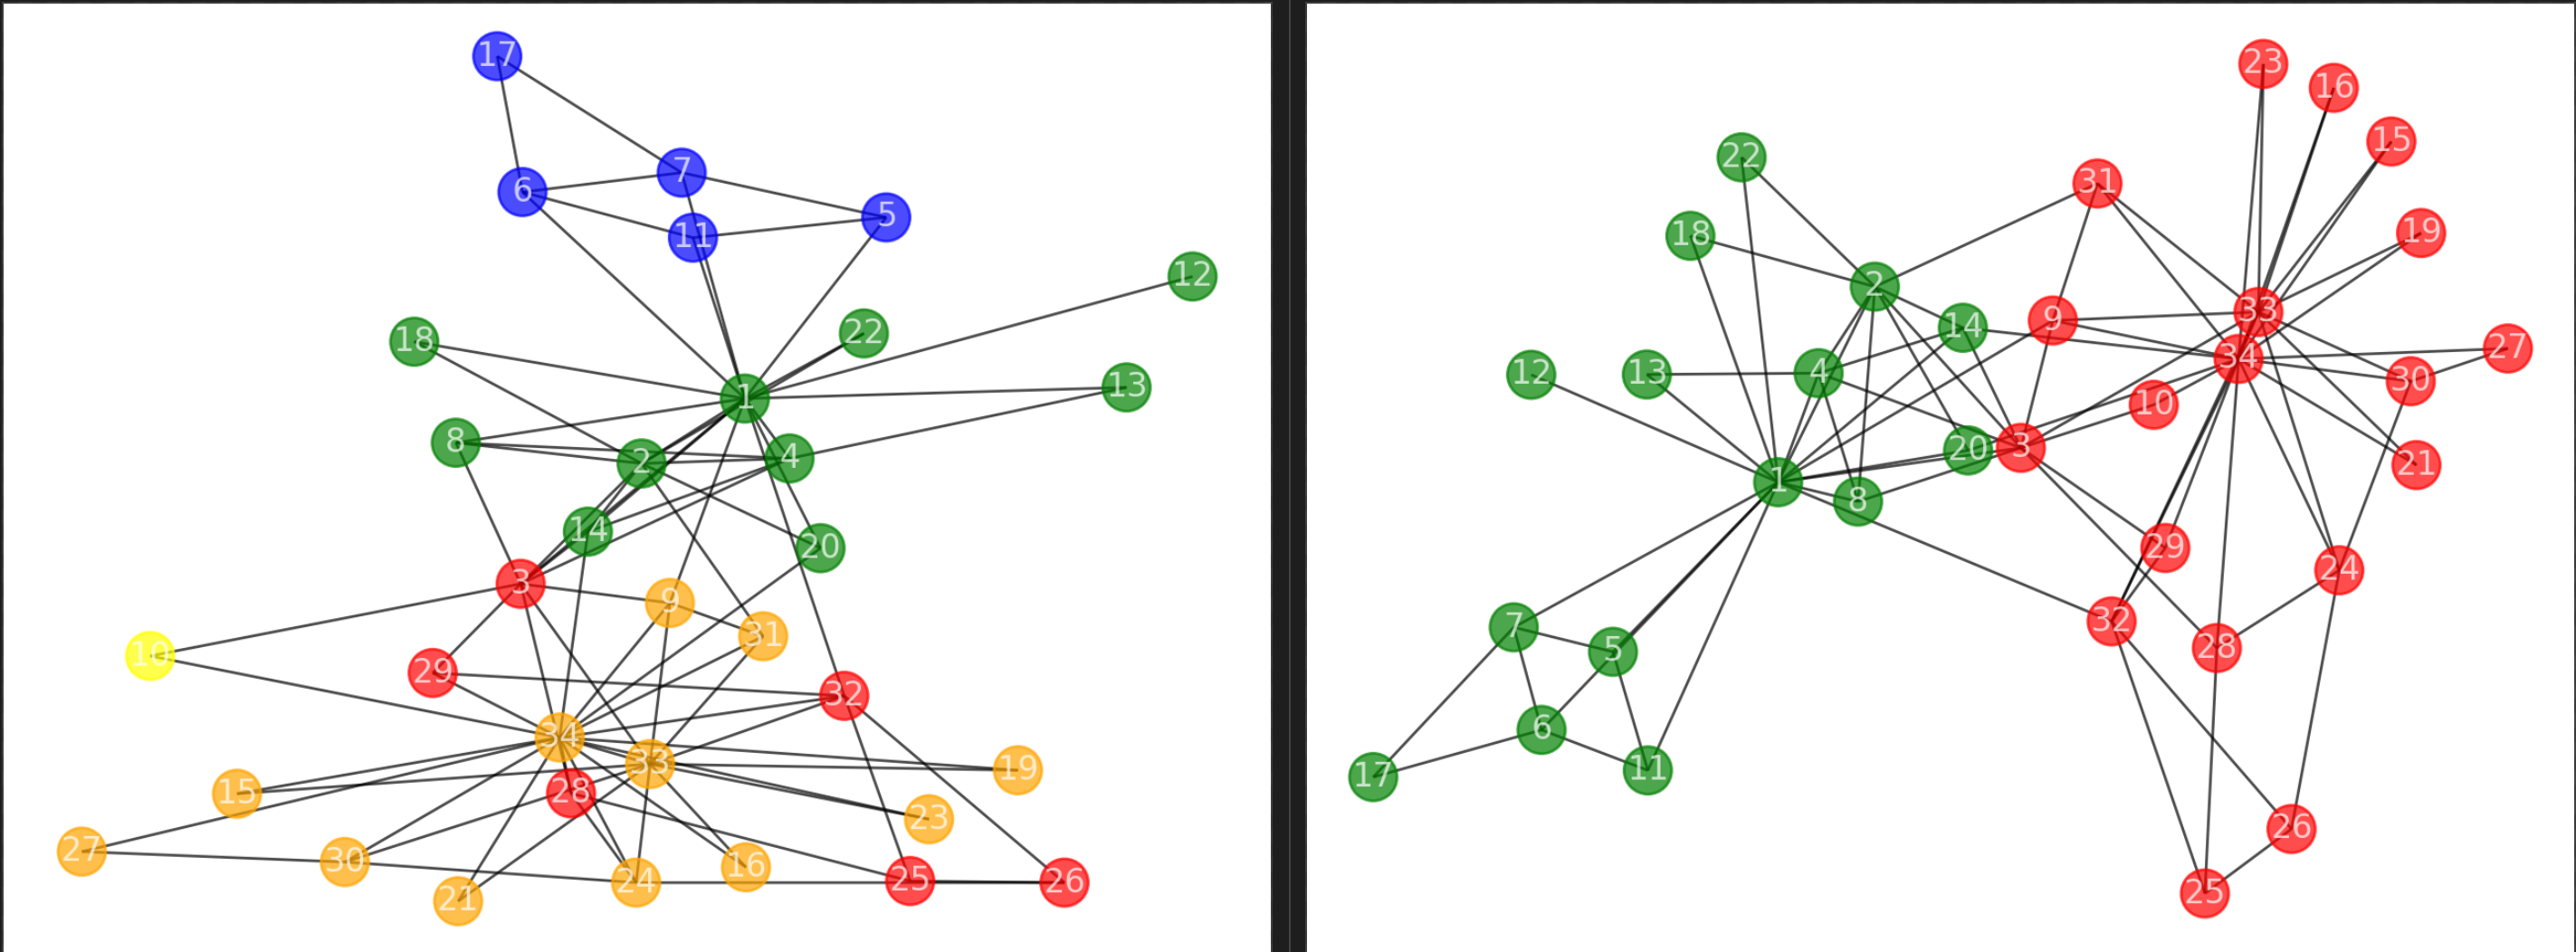
\includegraphics[scale=0.21]{Karate_GN_basic_vs_density.png}
\end{center}
\caption{Sa leve strane slike je podrazumevani GN, dok je sa desne strane GN sa gustinskom modularnošću sa parametrom $\lambda$=0.3}
\label{fig:GN1}
\end{figure}
\end{frame}

\begin{frame}\frametitle{Karate Club}
\begin{figure}[h!]
\begin{center}
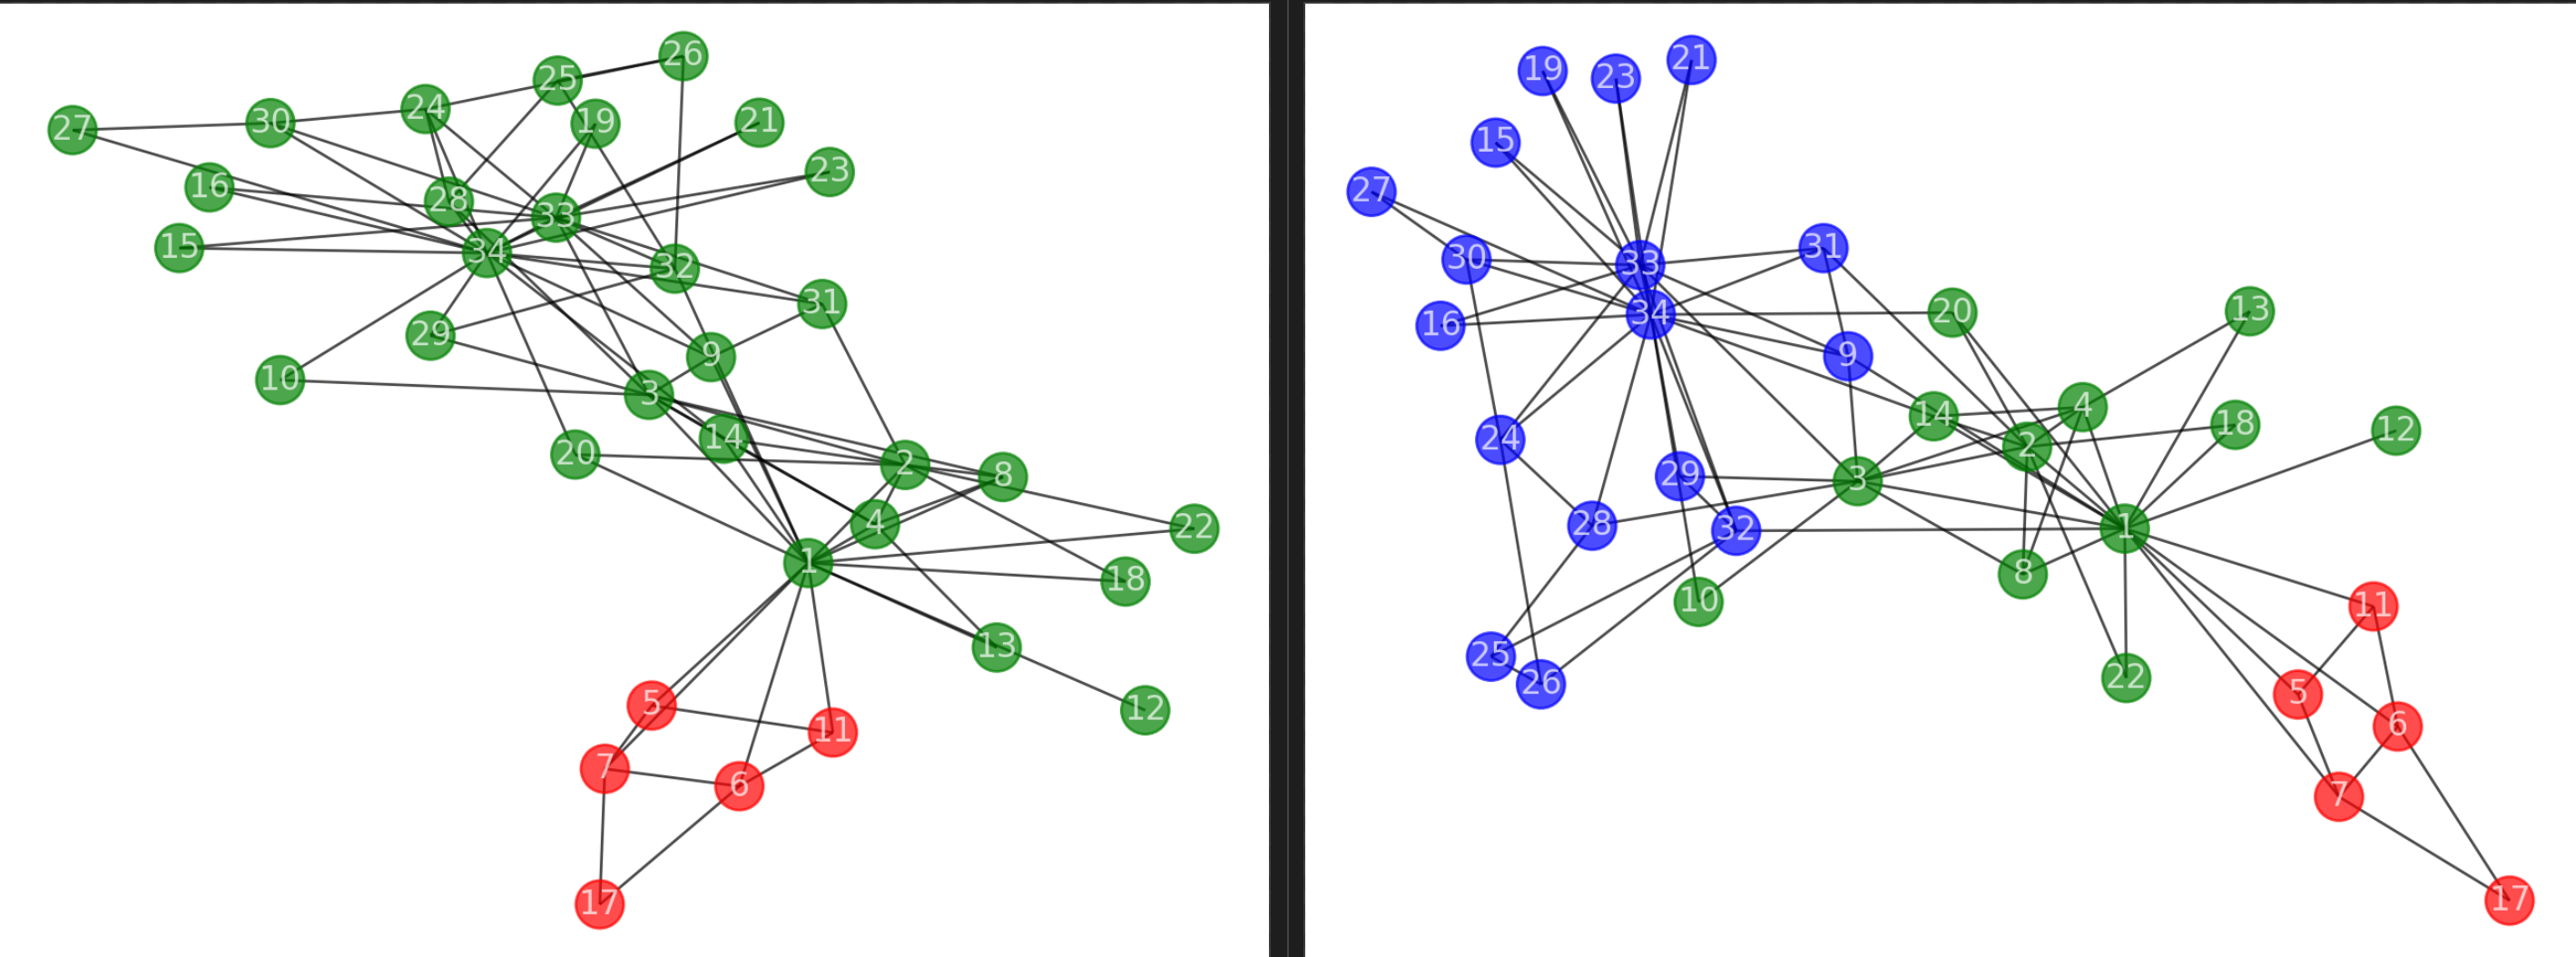
\includegraphics[scale=0.21]{Karate_MA_Local_vs_SAnnealing_20_generations.png}
\end{center}
\caption{Sa leve strane slike je Meme-Net, dok je sa desne strane Meme-Net sa simuliranim kaljenjem (oba za 20 generacija) i $\lambda$=0.5}
\label{fig:Meme1}
\end{figure}
\end{frame}

\begin{frame}\frametitle{Karate Club}
\begin{figure}[h!]
\begin{center}
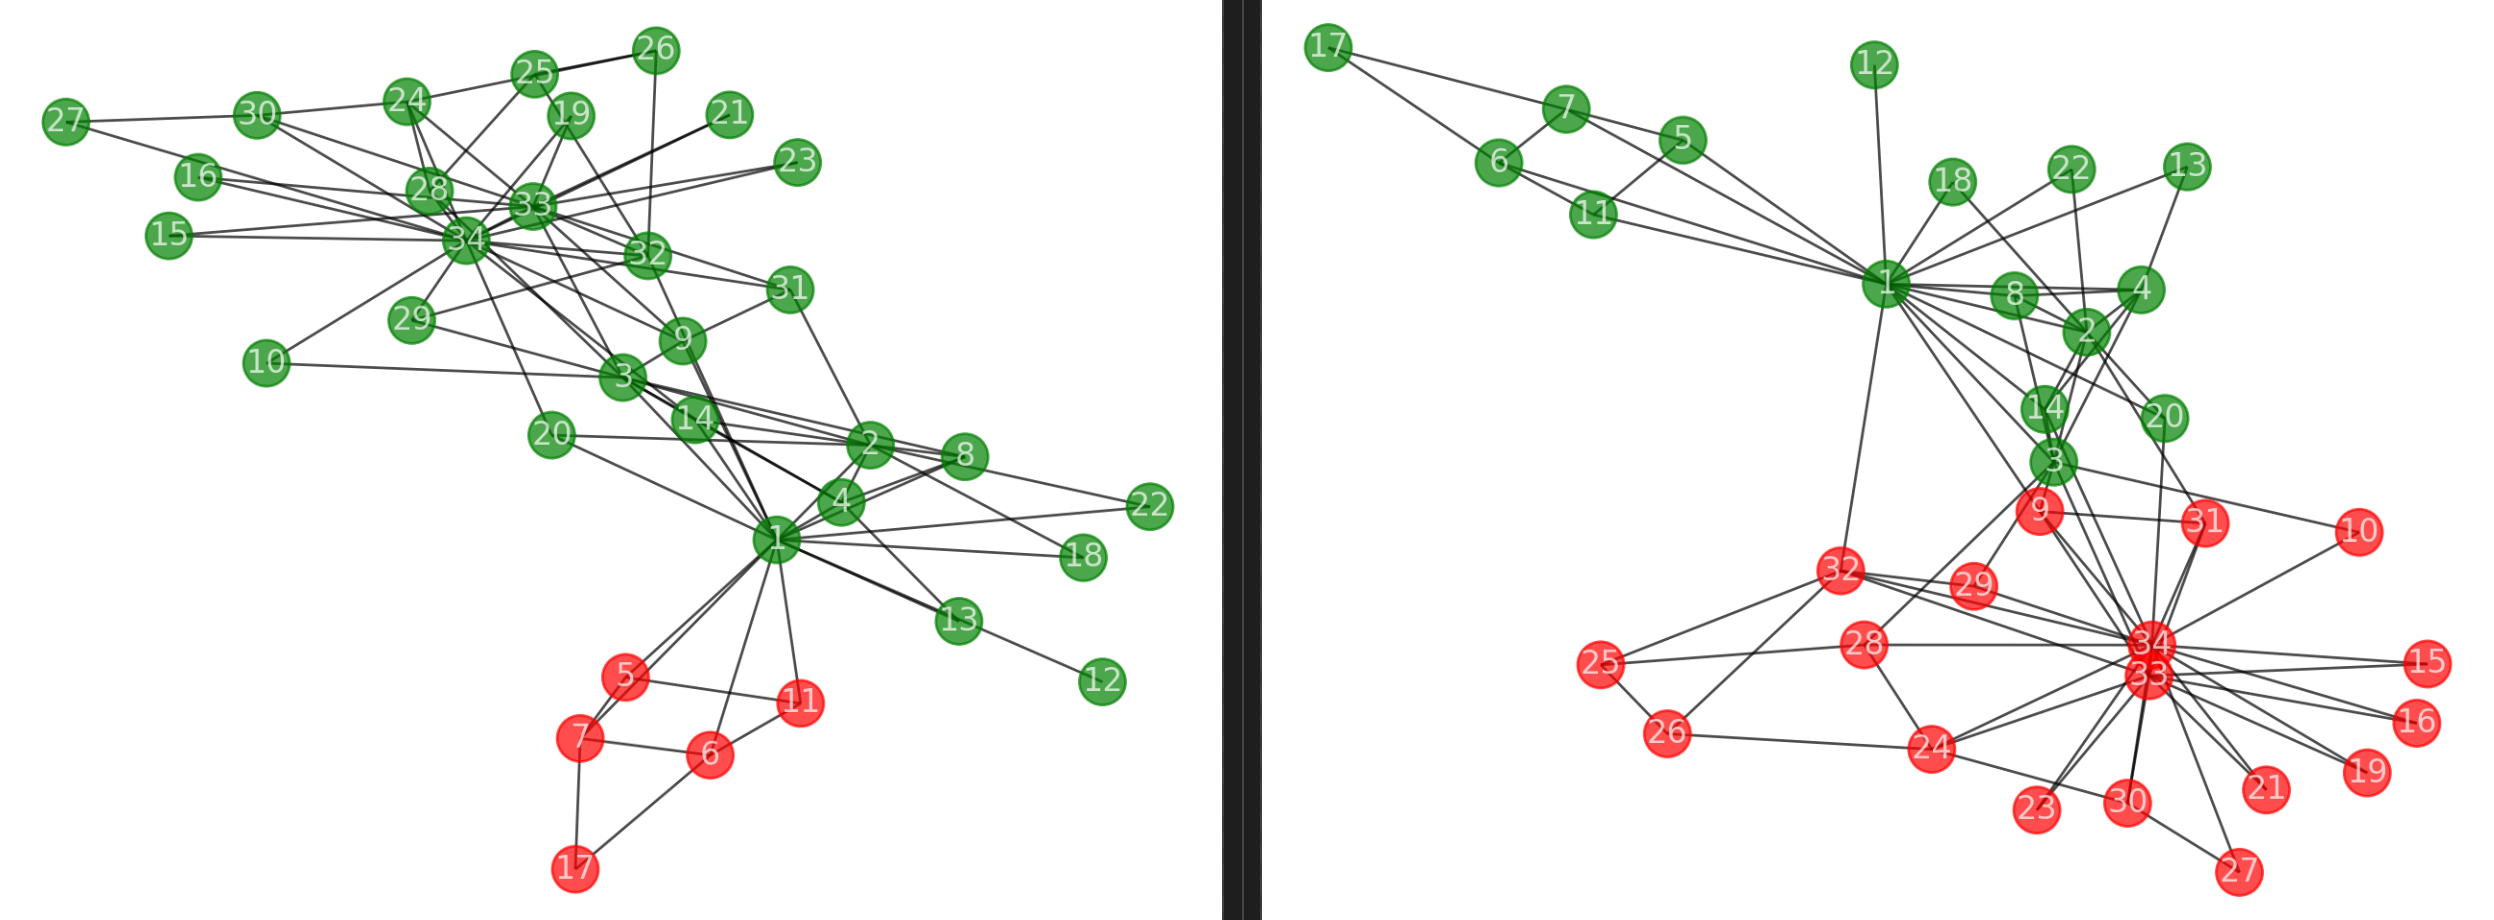
\includegraphics[scale=0.23]{GN3_comparing.png}
\end{center}
\caption{Sa leve strane slike je Meme-Net, dok je sa desne strane Meme-Net sa simuliranim kaljenjem (oba za 20 generacija) i $\lambda$=0.3}
\label{fig:Meme2}
\end{figure}
\end{frame}

\subsection{Dolphins}
\begin{frame}\frametitle{Dolphins}
\begin{figure}[h!]
\begin{center}
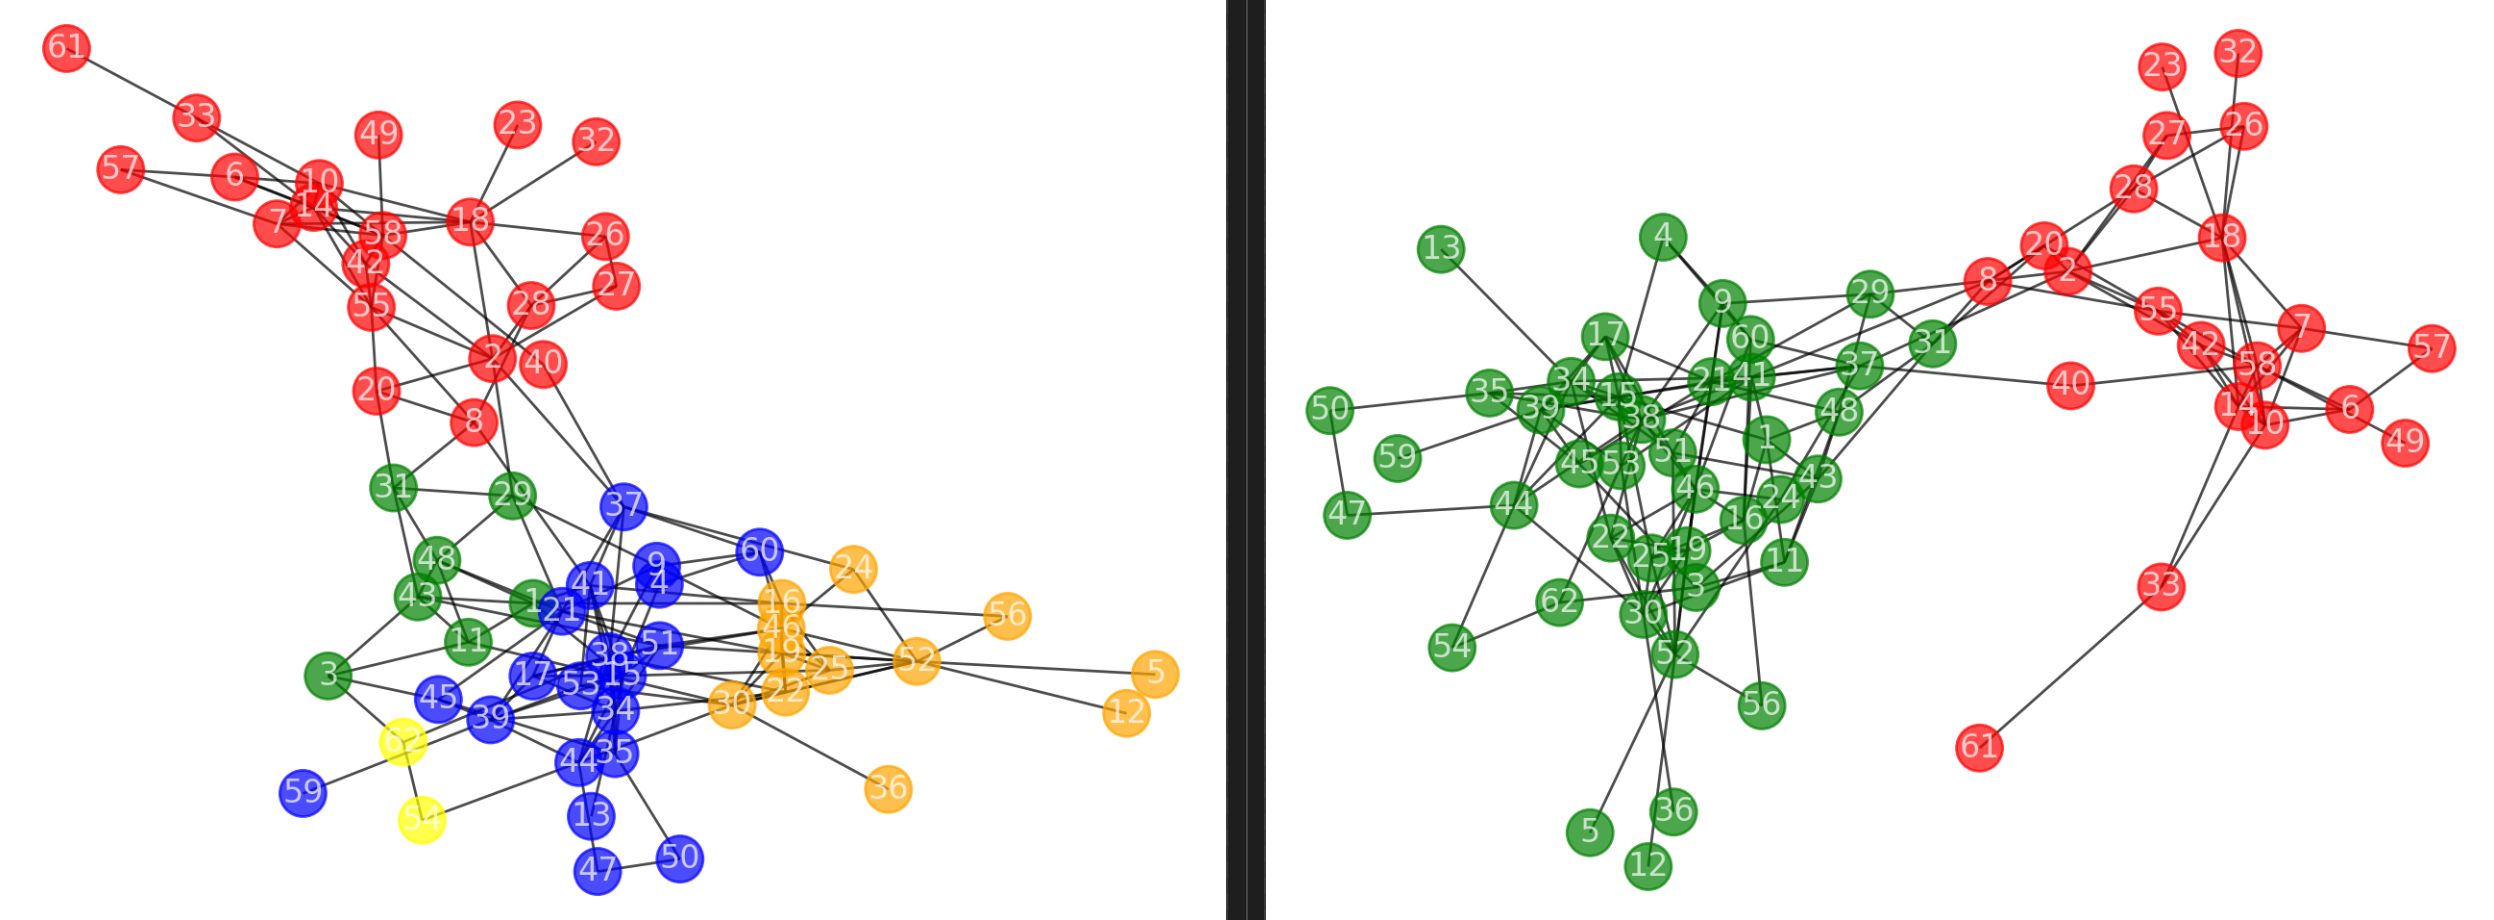
\includegraphics[scale=0.23]{GN_dolphins1.png}
\end{center}
\caption{Sa leve strane slike je podrazumevani GN, dok je sa desne strane GN sa gustinskom modularnošću sa parametrom $\lambda$=0.3.}
\label{fig:GN_Dolp_1}
\end{figure}
\end{frame}

\begin{frame}\frametitle{Dolphins}
\begin{figure}[h!]
\begin{center}
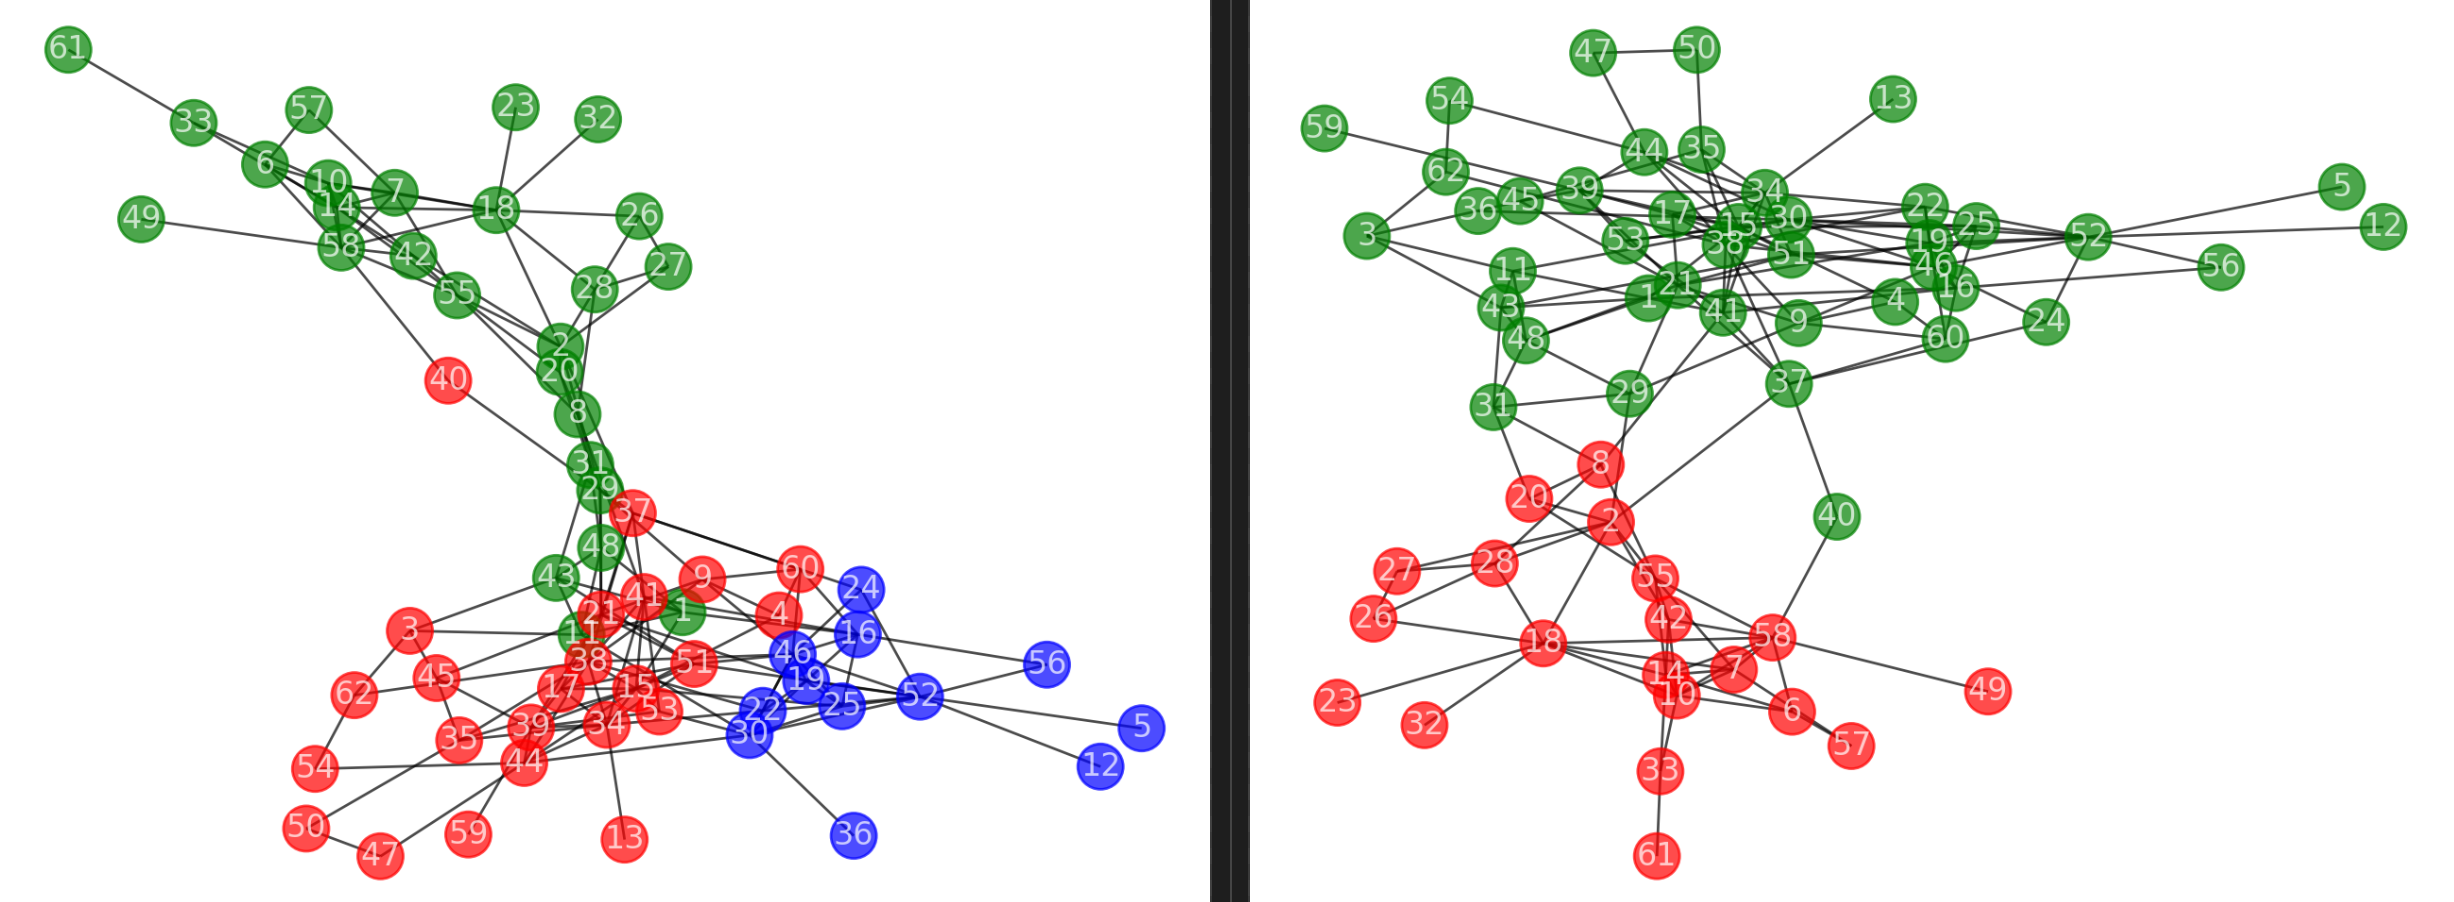
\includegraphics[scale=0.23]{MA_dolphin.png}
\end{center}
\caption{Sa leve strane slike je Meme-Net, dok je sa desne strane Meme-Net sa simuliranim kaljenjem (oba za 50 generacija) i $\lambda$=0.3}
\label{fig:Meme_dolp1}
\end{figure}
\end{frame}

\subsection{Jazz}
\begin{frame}\frametitle{Jazz}
\begin{figure}[h!]
\begin{center}
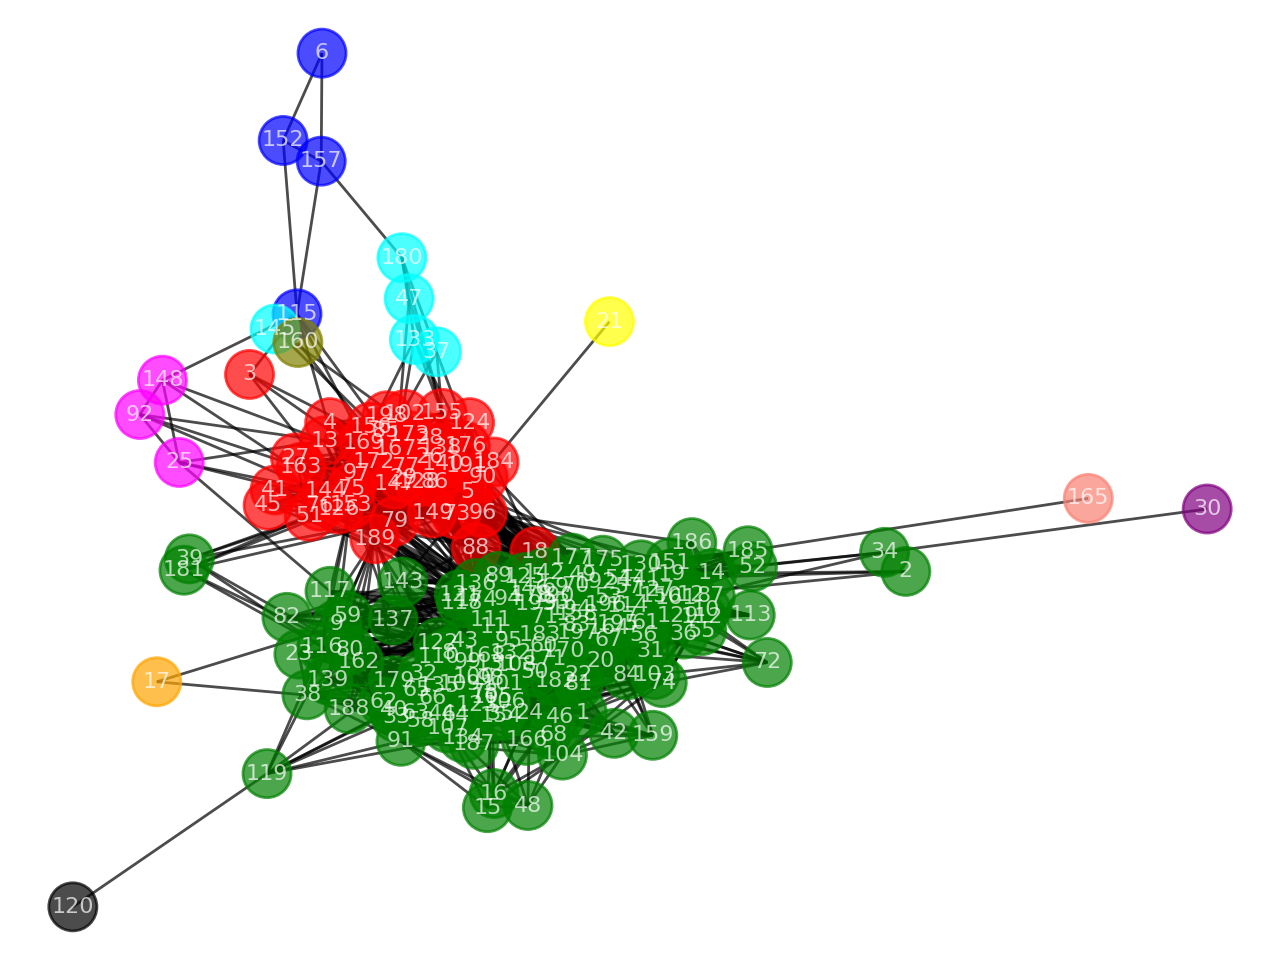
\includegraphics[scale=0.4]{Jazz_GN_0.7density.png}
\end{center}
\caption{GN sa gustinom $\lambda$=0.7}
\label{fig:Jazz_1}
\end{figure}
\end{frame}

\begin{frame}\frametitle{Jazz}
\begin{figure}[h!]
\begin{center}
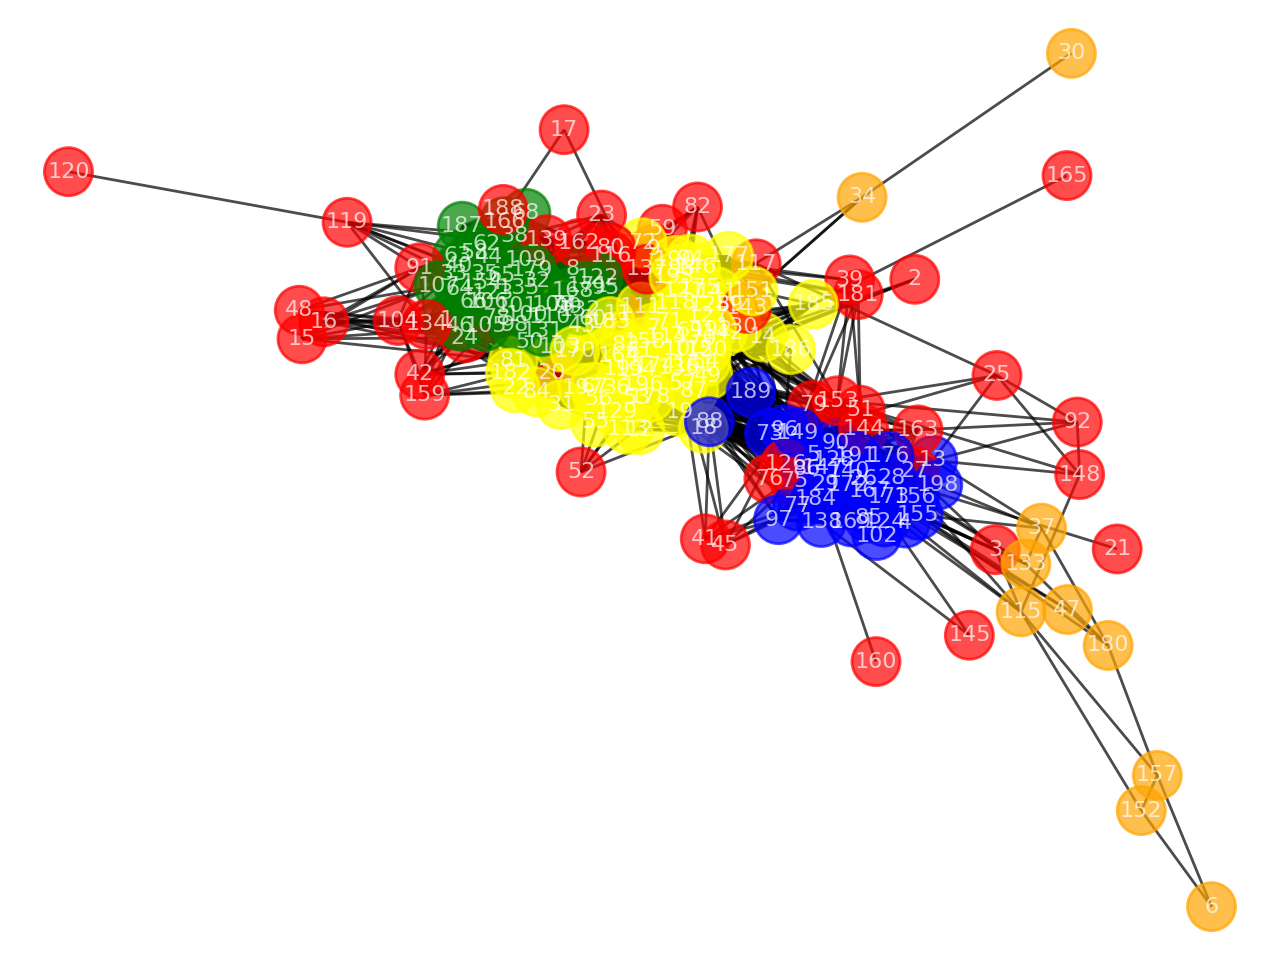
\includegraphics[scale=0.4]{Jazz_MA_local_100g_0.7density.png}
\end{center}
\caption{Meme-Net lokalna, 100 generacija, $\lambda$=0.7}
\label{fig:Jazz_2}
\end{figure}
\end{frame}

\begin{frame}\frametitle{Jazz}
\begin{figure}[h!]
\begin{center}
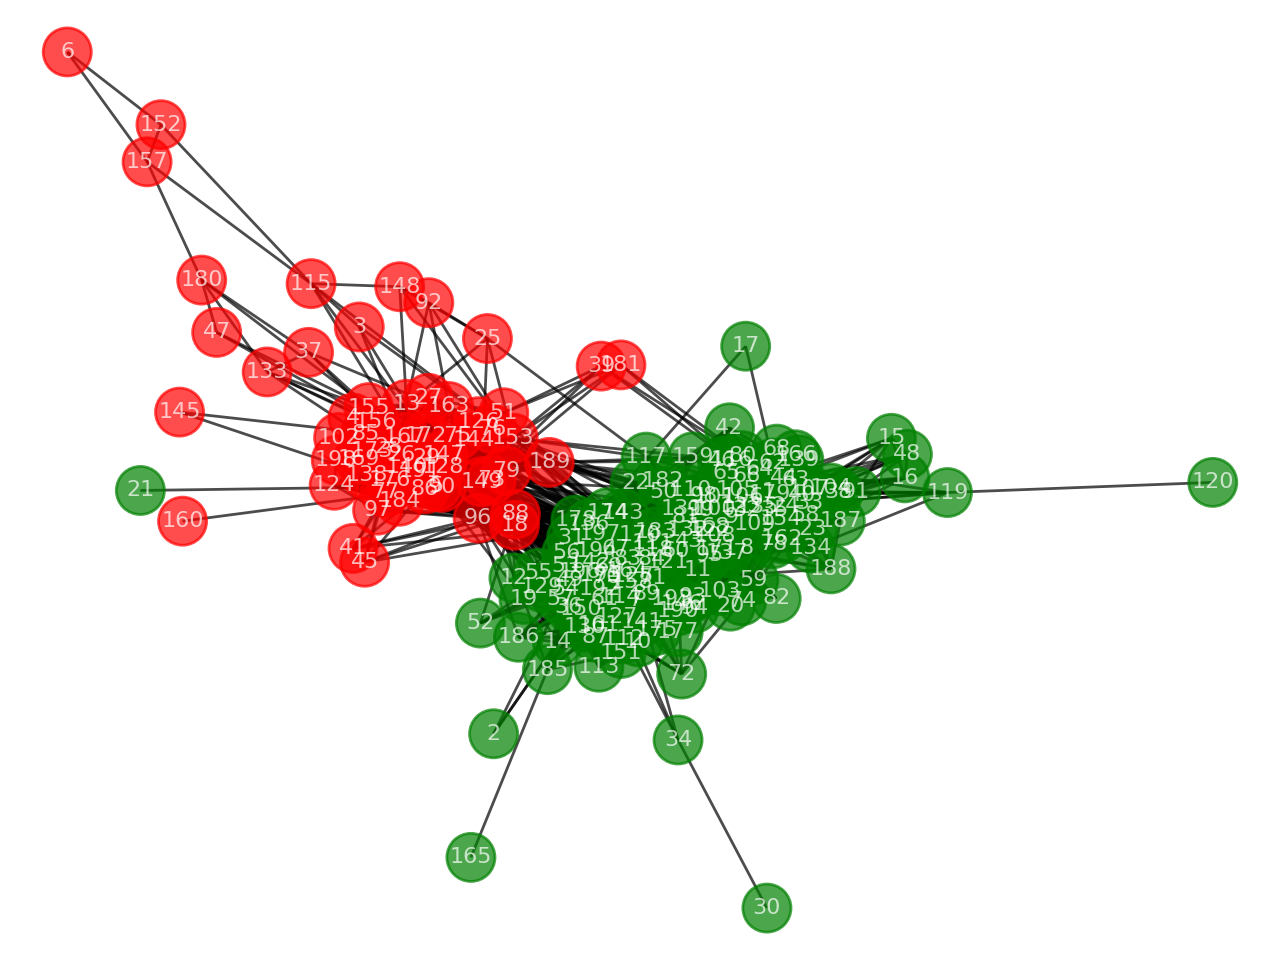
\includegraphics[scale=0.4]{Jazz_MA_SAnneal_100g_1000_0.7density.png}
\end{center}
\caption{Meme-Net simulirano, 100 generacija, $\lambda$=0.7}
\label{fig:Jazz_3}
\end{figure}
\end{frame}

\section{Diskusija i zaključak} 
\begin{frame}\frametitle{Diskusija i zaključak} 
\begin{itemize}
    \item ponašanje algoritma zavisi od problema
    \item rezlutati istraživanja pokazuju prednost gustinske modularnosti u odnosu na klasičnu (kod Girvan-Newman algoritma)
    \item za ispitane slučajeve konvergencija je brža ukoliko se koristi simulirano kaljenje, što ne mora biti opšti obrazac ponašanja (kod Meme-Net algoritma)
    \item dalji fokus istraživanja može biti primena ovih algoritama na veće zajednice, kao i testiranje u više istih iteracija kako bi se izvukao prosek 
\end{itemize}

\end{frame}

\section{Pitanja?}
\begin{frame}
Hvala na pažnji.
\newline
\vspace{30pt}Pitanja?
\end{frame}

\setbeamertemplate{footline}{\hspace*{.5cm}\scriptsize{\hspace*{50pt} \hfill\hspace*{.5cm} \setbeamercolor{black}}\\
\vspace{9pt}}

\setbeamertemplate{headline}{\hspace*{.5cm}\scriptsize{\hspace*{50pt} \hfill\hspace*{.5cm} \setbeamercolor{black}}\\
\vspace{1pt}}

%\setbeamercolor{mysection in head/foot}{bg= black,fg=black}

\end{document}